\begin{center}
    \textbf{Geração 40}
\end{center}

\begin{figure}[h]
    \centering
    \label{fig:geracao01}
    
    \begin{tabular}{rl}
        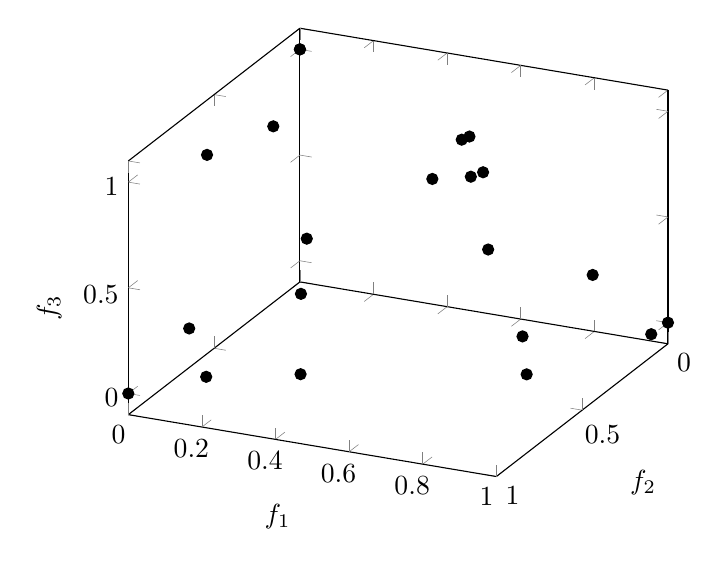
\begin{tikzpicture}[scale=1.0]
        	\begin{axis}[xlabel=$f_2$, ylabel=$f_1$, zlabel=$f_3$, view/h=115]
    			\addplot3[only marks] coordinates {
            		(1.000000, 0.000000, 0.000000) (0.000000, 1.000005, 0.000000) (0.541310, 0.000000, 0.840826) (0.000000, 0.000000, 1.000000) (0.000000, 0.000000, 1.000100) (0.690770, 0.340668, 0.638039) (0.440888, 0.717065, 0.540097) (0.283763, 0.596710, 0.750610) (0.972652, 0.198867, 0.120003) (0.503432, 0.839569, 0.204175) (0.804128, 0.377736, 0.459023) (0.392292, 0.110508, 0.914662) (0.174991, 0.521211, 0.835300) (0.361131, 0.528193, 0.768503) (0.088933, 0.996042, 0.000000) (0.940498, 0.137695, 0.310651) (0.515189, 0.856284, 0.036855) (0.245252, 0.612009, 0.751863) (0.238386, 0.906635, 0.348119) (0.147666, 0.529444, 0.835399) (0.895597, 0.419339, 0.148531) 

        		};
        	\end{axis}
	    \end{tikzpicture}
	    &
	    \begin{tikzpicture}[scale=1.0]
        	\begin{axis}[xlabel=$f_2$, ylabel=$f_1$, zlabel=$f_3$, view={45}{0}]
    			\addplot3[only marks] coordinates {
            		(1.010984,0.000000,0.000000)(0.000000,1.037529,0.000000)(0.000000,0.000000,1.030206)(0.000000,0.000000,1.074789)(0.665893,0.744773,0.198561)(0.673572,0.401364,0.663685)(0.218021,0.889701,0.405159)(0.513301,0.088910,0.923083)(0.957956,0.134562,0.265313)(0.079043,1.020902,0.040988)(0.393249,0.981370,0.000000)(0.144434,0.613702,0.831113)(0.842780,0.278098,0.542046)(0.637467,0.308309,0.774694)(0.942479,0.004177,0.474421)(0.838668,0.546414,0.168372)(0.070071,0.673875,0.775207)(0.308683,0.940953,0.320588)(0.254647,0.924109,0.389850)(0.764959,0.478170,0.601281)(0.843468,0.511611,0.251668) 

        		};
        	\end{axis}
	    \end{tikzpicture}
	\end{tabular}
    
\end{figure}

